\section{Online Census}

The advent of mobile sensing techniques and social media applications makes it possible to collect spatial data from the social media source. Complementary to the conventional census, it brings the benefit of larger sampling frequency and a broader range in terms of space and time. It is possible to reach a wide range of individuals and collect the movement in human inactive time, such as the mid-night.


\begin{figure}[htb!]
 \centering % avoid the use of \begin{center}...\end{center} and use \centering instead (more compact)
 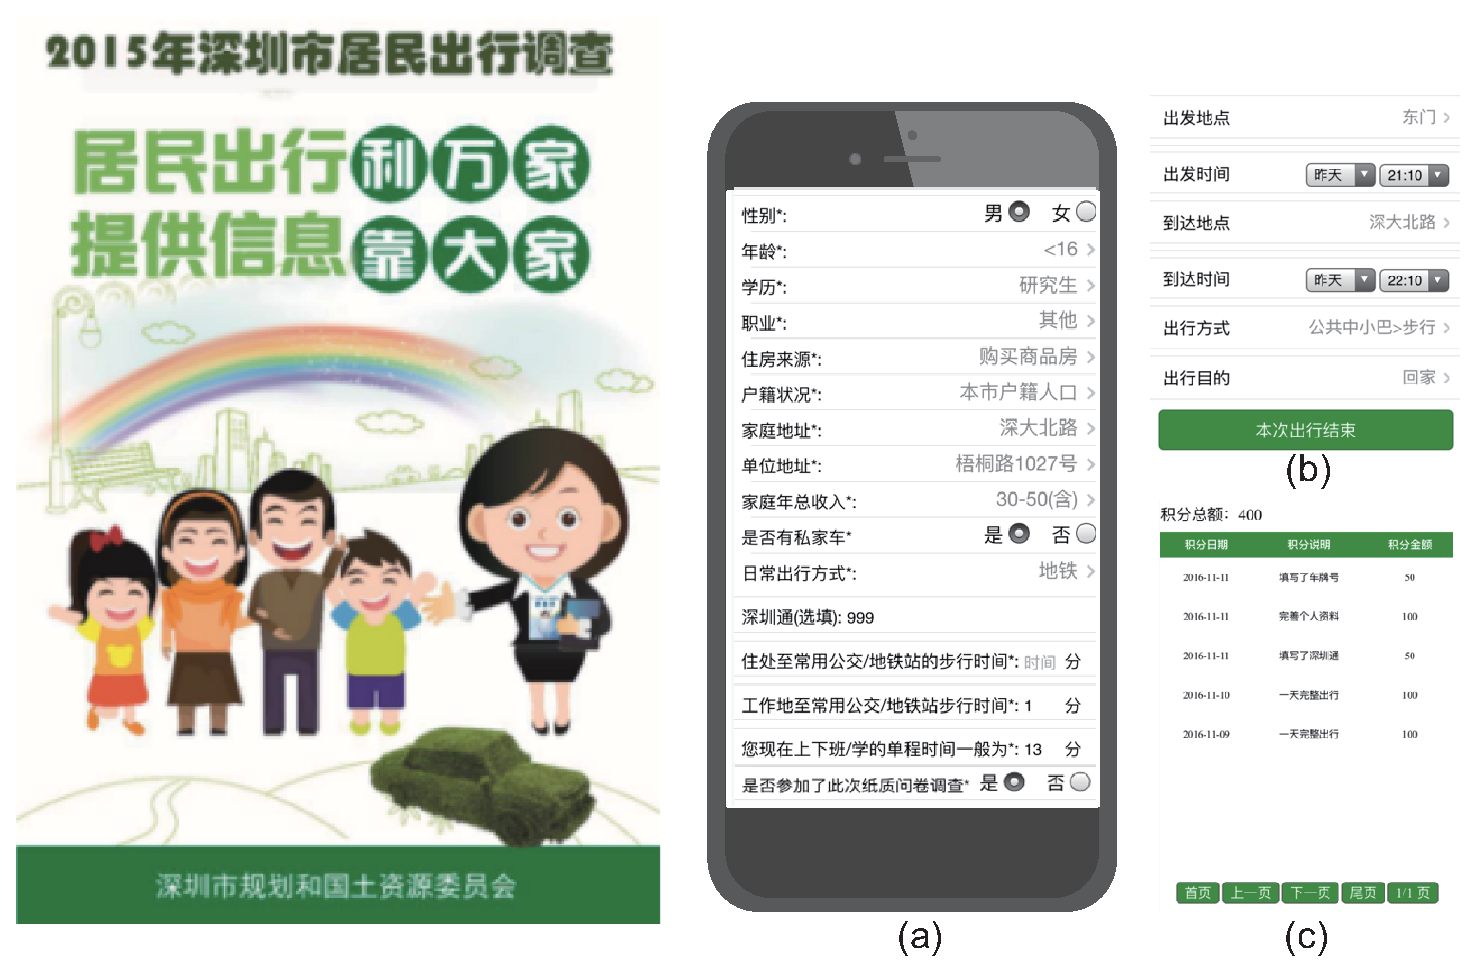
\includegraphics[width=\columnwidth]{pictures/survey_app}
 \caption{Census Interface: (a) personal characteristics collecting page; (b) trips collecting page; (c) credit system page}
 \label{fig:app}
\end{figure}

In this work, we perform the census survey in Shenzhen, which is one of the most modern metropolia in China. The experiment is deployed on Wechat, a widely used social media application. Figure~\ref{fig:app} shows the data collecting interfaces. Each individual hands in his or her personal characteristics. For privacy issue, all detailed personal information are desensitized to categorical levels (Figure~\ref{fig:app}(a)). 


\textbf{Individual Characteristics} Figure~\ref{fig:data_over} lists the \textit{eight domains}, including social, economic and demographic aspects, to give a generalized description of the individual characteristics. The profile will serve as the ingredients for the analysis of mobility patterns over diverse individuals. 


\begin{figure}[htb!]
 \centering % avoid the use of \begin{center}...\end{center} and use \centering instead (more compact)
 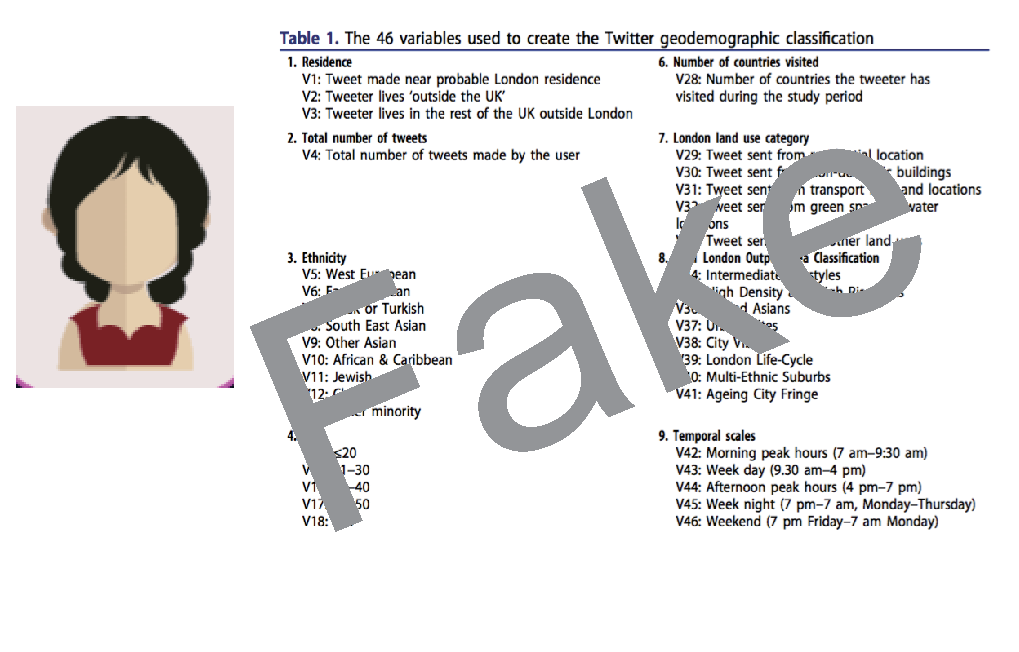
\includegraphics[width=\columnwidth]{pictures/data_over}
 \caption{Profile of Individual: eight individual characteristics enrich the analysis of mobility patterns}
 \label{fig:data_over}
\end{figure}

\textbf{Traveling Trips} Besides to those individual characteristics, each individual can upload dynamic traveling trips (Figure~\ref{fig:app}(b)). Each trip requires the information of \textit{start/end location}, \textit{start/end time}, \textit{traveling purpose}. To encourage the trip uploading, a credit system retains the contribution of individuals on trips and rewards the volunteers with the top credits (Figure~\ref{fig:app}(c)). 


\subsection{Basic Statistics of Data}

Over the releasing time period from \m{2015-11 to 2016-01}, 21435 individuals (48\% females and 52\% males) were reached and \m{229155} trips are collected. Each volunteer contributes \m{11} trips average. 

Our case-study data is confined to a small proportion of Wechat users who opt to contribute their information and trips.
Considering the caveat that self-selecting individuals are most unlikely to represent any clearly defined population~\cite{Longley2015}, we performed a series of preliminary statistics to check whether it is rich enough to represent a wide range of the population in the city. 

Figure~\ref{fig:data_age_edu} gives the distribution of age and education over the population. It shows that samples cover a wide range of ages, dominating between 18 to 45. There is also a few records pertaining to individuals below the age of 18 or above 70. The distribution follows the fact that Shenzhen is a city where the majority is young people. According to the 2015 Annual Census Statistics report\footnote{http://www.sztj.gov.cn/xxgk/tjsj/pcgb/201606/t20160614\_3697000.htm}, people aging 15-64 occupy 83.23\% and the median age is 31.5. Figure~\ref{fig:data_age_edu} gives the distribution of education levels, ranging from low to high. The technical college and university dominate the samples at the 61\% occupancy rate. 

% In the report (looking for some report), the penetration of mobile device is \m{XXX}, almost every XX people got a Mobile Phone in the urban. 

\begin{figure}[htb!]
 \centering % avoid the use of \begin{center}...\end{center} and use \centering instead (more compact)
 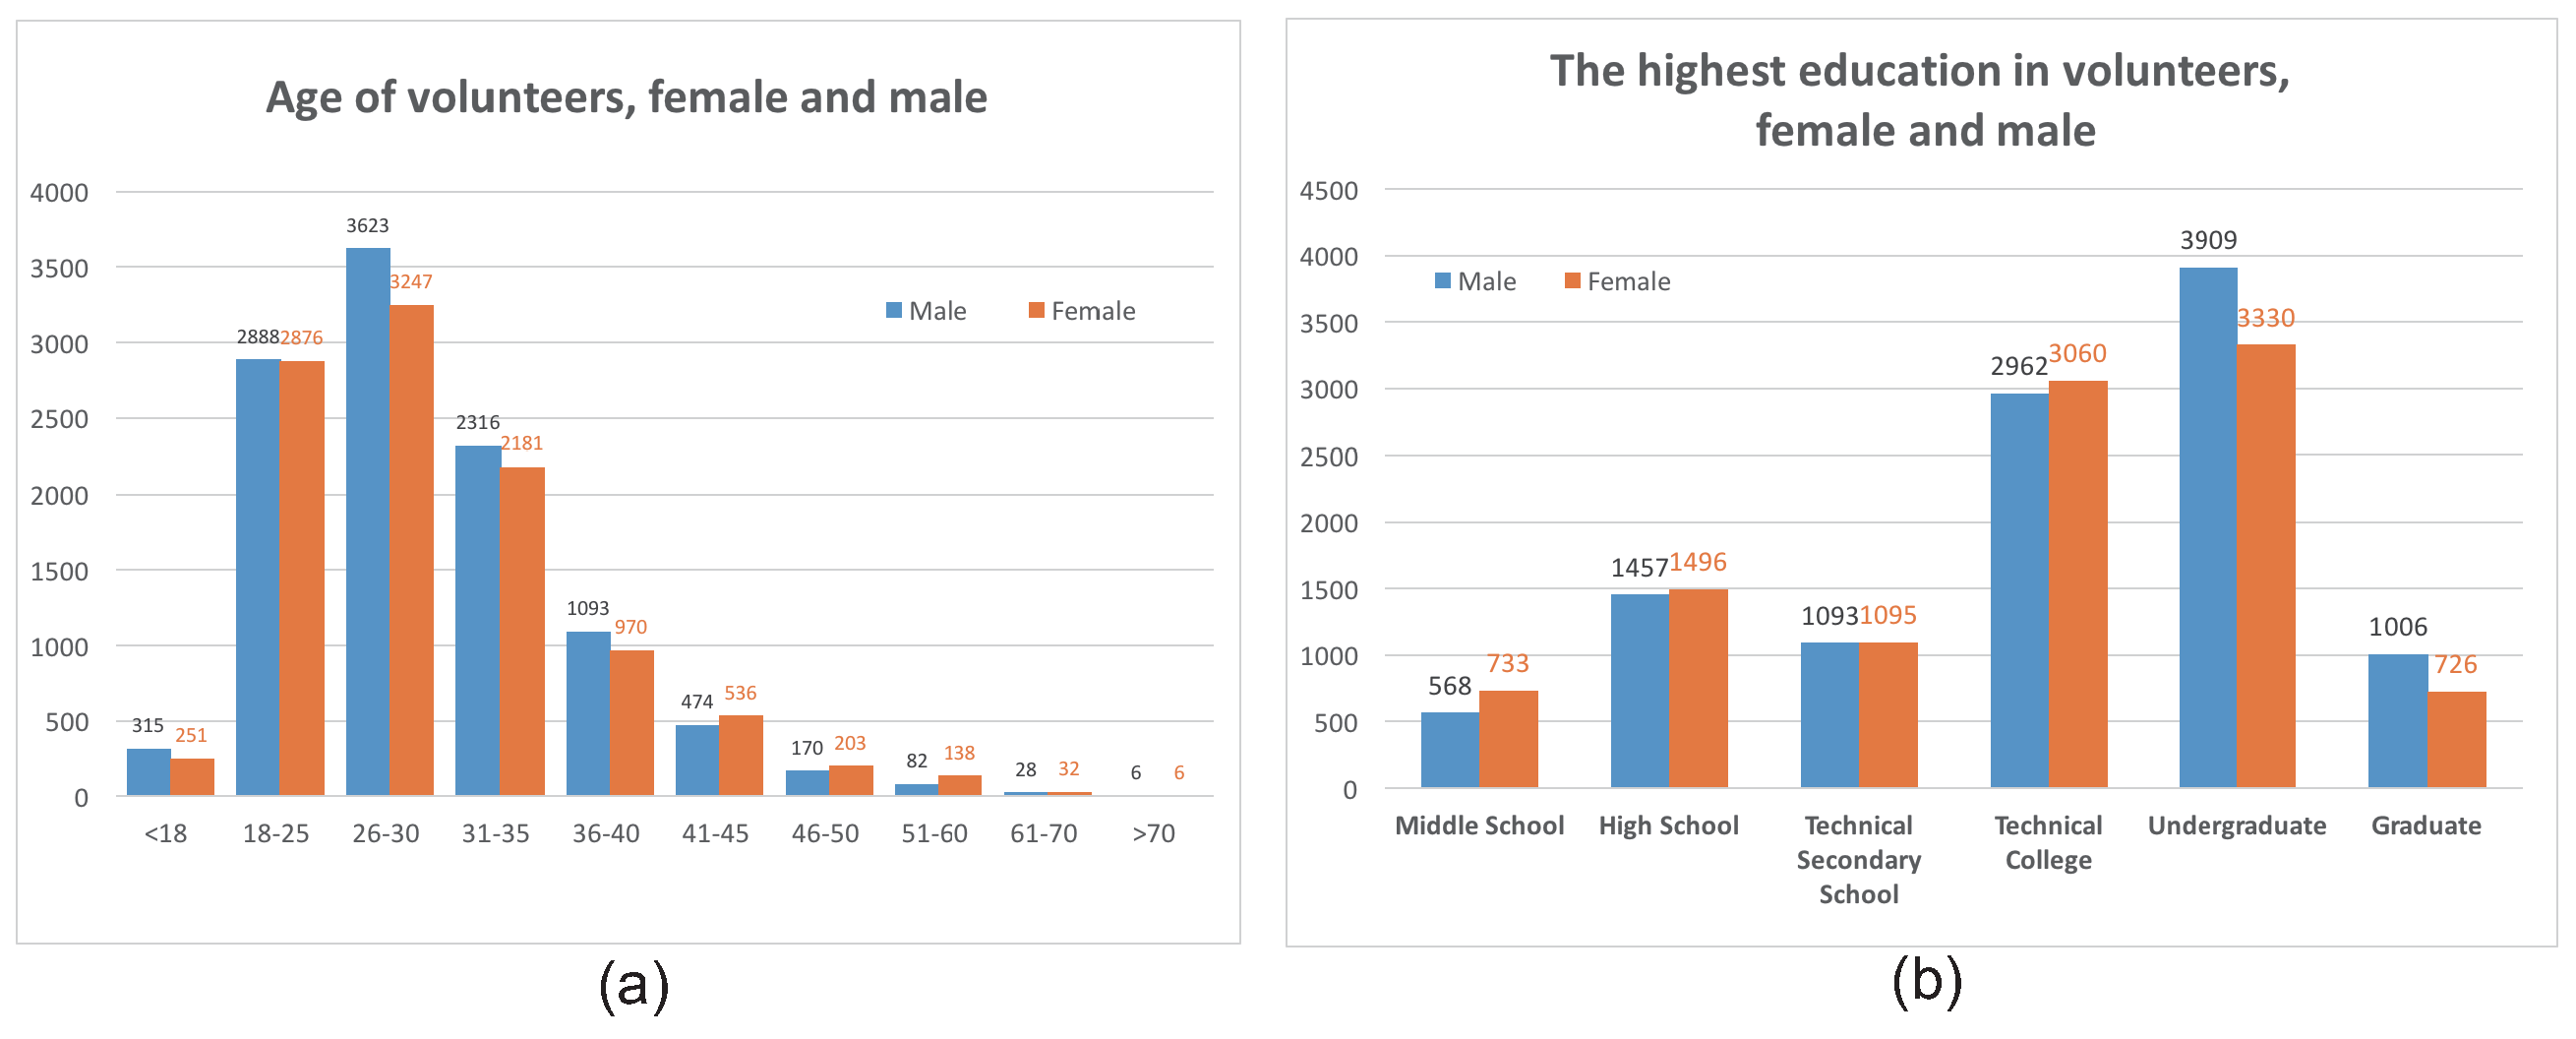
\includegraphics[width=\columnwidth]{pictures/data1}
 \caption{Age and Education Distribution: (a) age; (b) education}
 \label{fig:data_age_edu}
\end{figure}

Figure~\ref{fig:data_job_inc}(a) shows the job types of sampled individuals, who are servants, workers, officers, businessmen and so on. The covering of jobs is pretty wide. Figure~\ref{fig:data_job_inc}(b) gives the radar diagram of the annual pay. The majority get paid below 200 000. Individuals with higher salary are also reached in our census.

\begin{figure}[htb!]
 \centering % avoid the use of \begin{center}...\end{center} and use \centering instead (more compact)
 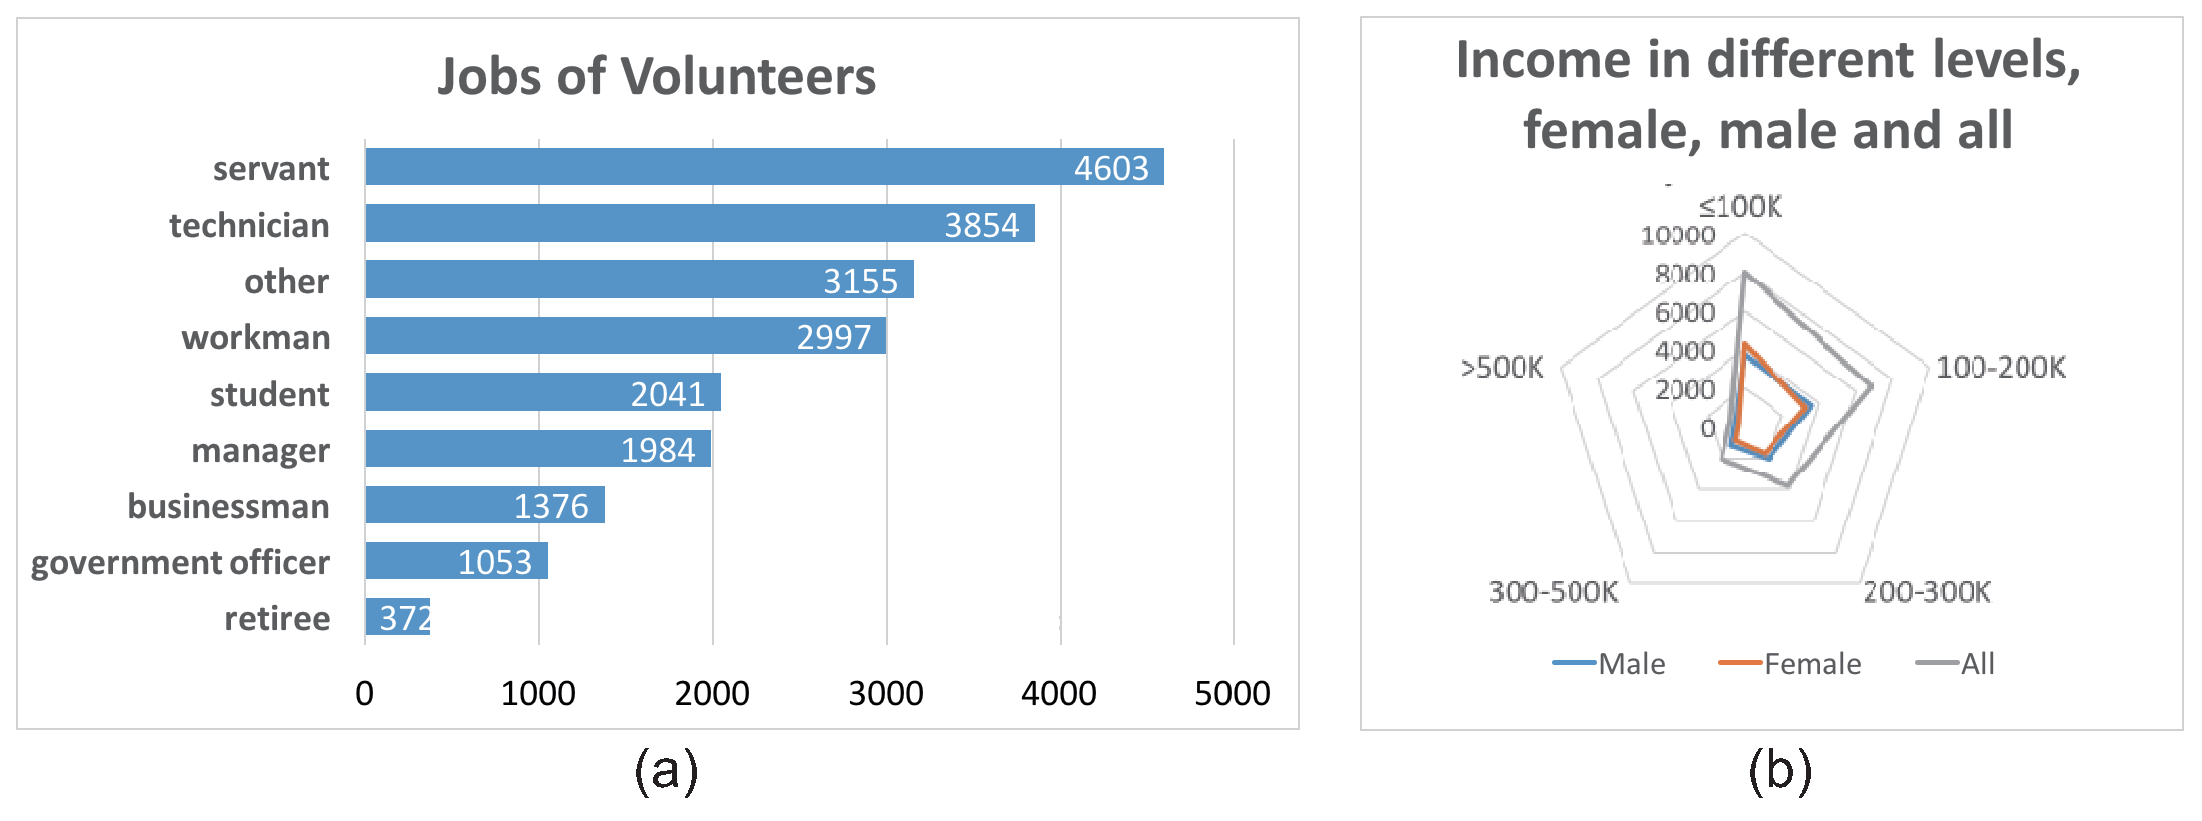
\includegraphics[width=\columnwidth]{pictures/data2}
 \caption{Job and Income Distribution: (a) job; (b) income}
 \label{fig:data_job_inc}
\end{figure}

Figure~\ref{fig:data_geometry} shows the basic statistics related to trips. In Figure~\ref{fig:data_geometry}(a), the active traveling time (here, we take the start time as the representative of active time) follows the common knowledge of urban life. There are obvious morning and late afternoon peaks. Figure~\ref{fig:data_geometry}(b) gives the counting of different traveling purposes. 95\% trips are tagged with clear raveling purpose in the data. 33\% are going home and 37\% are going to work. Besides this kind of routine traveling, there are also substantial trips such as going shopping, going the hospital, etc. Figure~\ref{fig:data_geometry}(c) shows the spatial distribution of the origins and destinations. It is found that more dots are located in Futian and Nanshan districts, the city's heart than the surrounding areas. This is consistent to Batty's exposition of the focus of city networks and interaction patterns~\cite{batty2013new}. 

% Trips are uploaded in a wide range of purpose in addition to home, work, but also includes XX entertainment, visiting, etc. The diverse purposes make it possible to characterize the flows across the city between different functional places. 

\begin{figure}[htb!]
 \centering % avoid the use of \begin{center}...\end{center} and use \centering instead (more compact)
 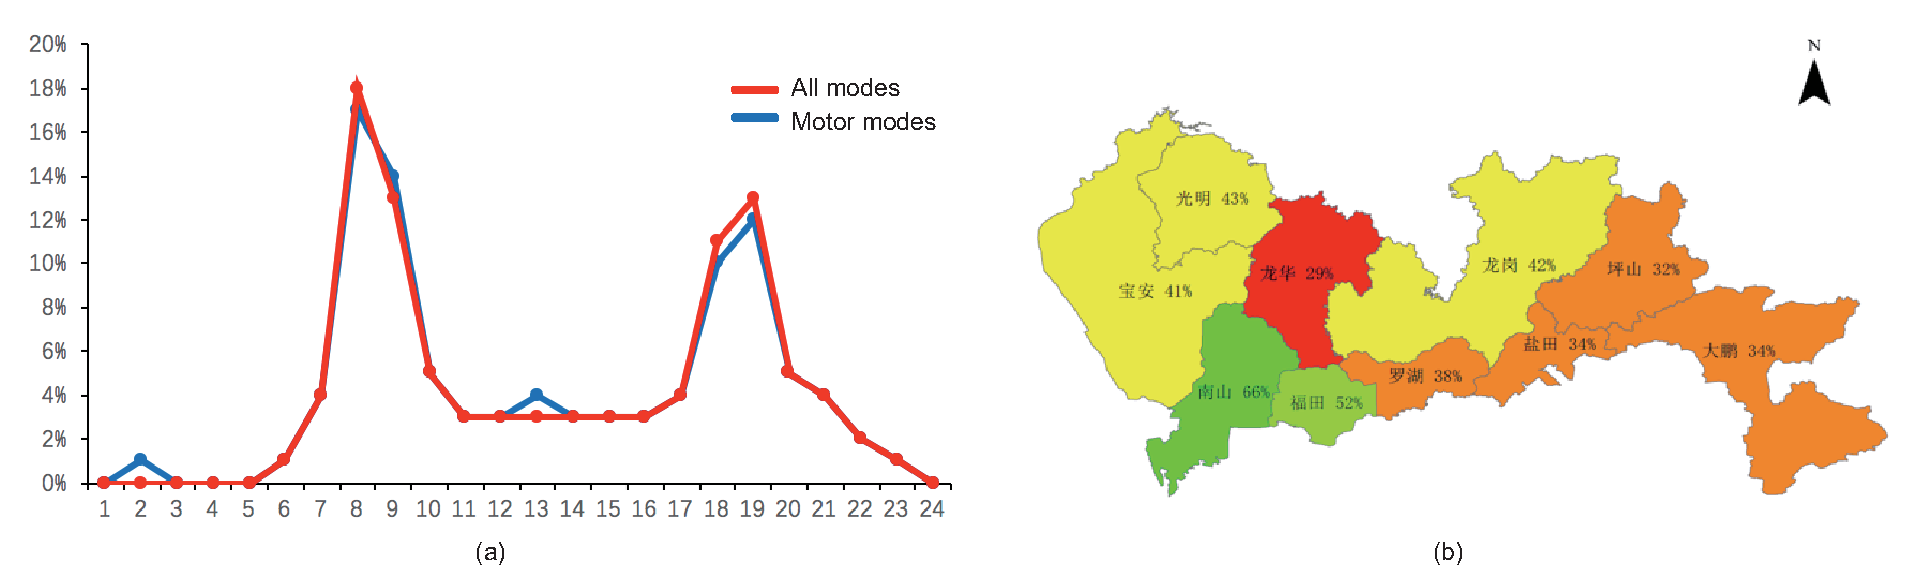
\includegraphics[width=\columnwidth]{pictures/data3}
 \caption{Statistics of Trips: (a) start time of trips; (b) purpose of trips; (c) distribution of origins/destinations }
 \label{fig:data_geometry}
\end{figure}

Because there is always inevitable bias inherent in fully representing the ground truth of the population, the preliminary statistical analysis shows positive sign of a relatively even sampling of the population. 
% As a note, although it is a subset of all people with 
